\chapter{Results}
This Chapter will outline the main results obtained with the two algorithms developed and tested as described in Chapter \ref{chapter:ML-PSD}. The various possible cuts, nameley the two of the \ac{VAE} and the three of the \ac{DTC}, will be applied to the calibration dataset in the 1550-1650 keV energy range, i.e. the one on which the algorithms are trained and tested, and on another novel dataset on which the networks have never been trained, the $2\nu\beta\beta$ spectrum from physics (\texttt{phy}) data of \textit{prl25}.

The deep learning cuts are compared with one another and with the traditional benchmark given by the \ac{AE} parameter (see Sec.~\ref{sec:traditionalPSD}). The comparison relies on two complementary analyses: the study of the events on which the traditional and the deep learning methods agree or disagree, and the \ac{AUC} of their \ac{ROC} curves, which quantifies the separation power of each method independently of the chosen cut threshold~\cite{ROCanalysis}.

\section{Analysis of calibration data}

\label{sec:calib-data}

\subsection{\texorpdfstring{\acs{VAE}}{VAE}-based classifier}
% \begin{figure}[H]
%     \centering
%     \includegraphics[width=0.8\textwidth]{plots/VAE/spectrum_cuts_sigma3_current_scaled_beta1.pdf}
%     \caption{\dots }
%     \label{fig:VAE-energyspectrum-3sigma}
% \end{figure}

% \begin{figure}[H]
%     \centering
%     \includegraphics[width=\textwidth]{plots/VAE/spectrum_cuts_sigma1_current_scaled_beta1.pdf}
%     \caption{\dots }
%     \label{fig:VAE-energyspectrum-1sigma}
% \end{figure}

\subsection{\texorpdfstring{\acs{DTC}}{DTC}}
\begin{wrapfigure}{r}{0.5\textwidth}
    \centering
    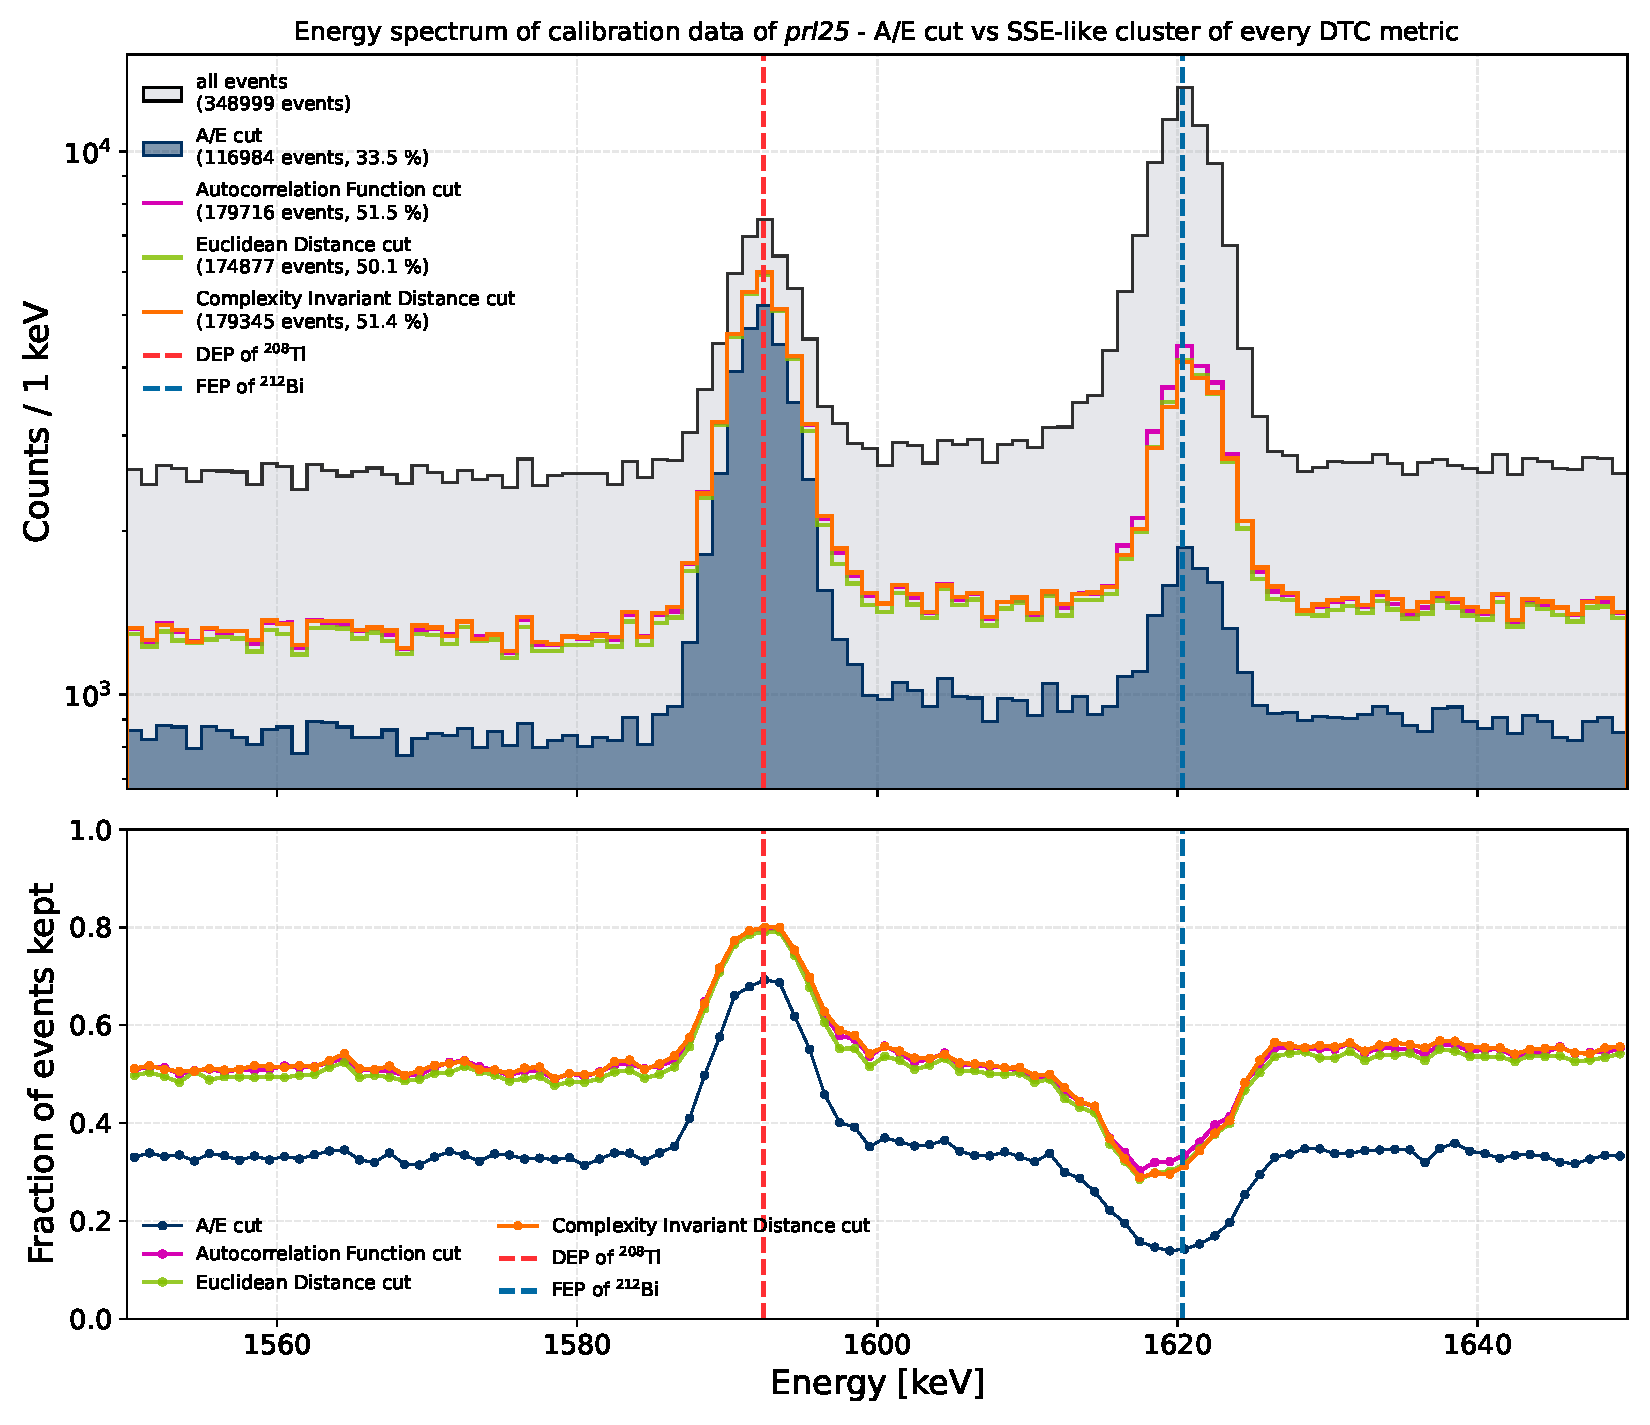
\includegraphics[width=\linewidth]{plots/DTC/calibrationData_wholeSpectrum/energy_spectrum_all_metrics_cuts.pdf}
    \caption{All metrics cuts on the whole calibration dataset.}
    \label{fig:DTC-energyspectrum-allmetrics}
\end{wrapfigure}
Figure~\ref{fig:DTC-energyspectrum-allmetrics} displays the three \ac{DTC} metrics cut on the calibration dataset for Euclidean Distance (green), Complexity Invariant Distance (orange) and Autocorrelation Function (purple). Moreover, the \ac{AE} cut is shown in blue to give a graphical comparison from which it is clear that the \ac{AE} cut is far less conservative with respect to the \ac{DTC} ones. Nonetheless, this aspect does not ensure the fact that the \ac{AE} parameter is a better solution to the \ac{SSE}-\ac{MSE} discrimination problem. Figure~\ref{fig:DTC-waveforms-allmetrics-agree} shows that it is evident that the waveforms both methods agree to retain are clearly \ac{SSE}-like events, whereas those they both reject exhibit distinct \ac{MSE}-like features. However Fig.~\ref{fig:DTC-waveforms-allmetrics-disagree} displays that the waveforms kept by the \ac{AE} but rejected by the \ac{DTC} include a lot of waveforms with multiple peaks typical of \ac{MSE} while the ones rejected by \ac{AE} but kept by the \ac{DTC} metrics are almost all \ac{SSE}-like events with only one peak and a simple structure. These comparisons highlight how a single parameter, i.e. \ac{AE}, cannot take into consideration the whole structure of a waveform and therefore may lead to an unproper \ac{SSE}-\ac{MSE} discrimination, while the \ac{DTC} model can perform this distinction better, seeing that it considers the whole time series of a waveform.

% \begin{figure}[H]
%     \centering
%     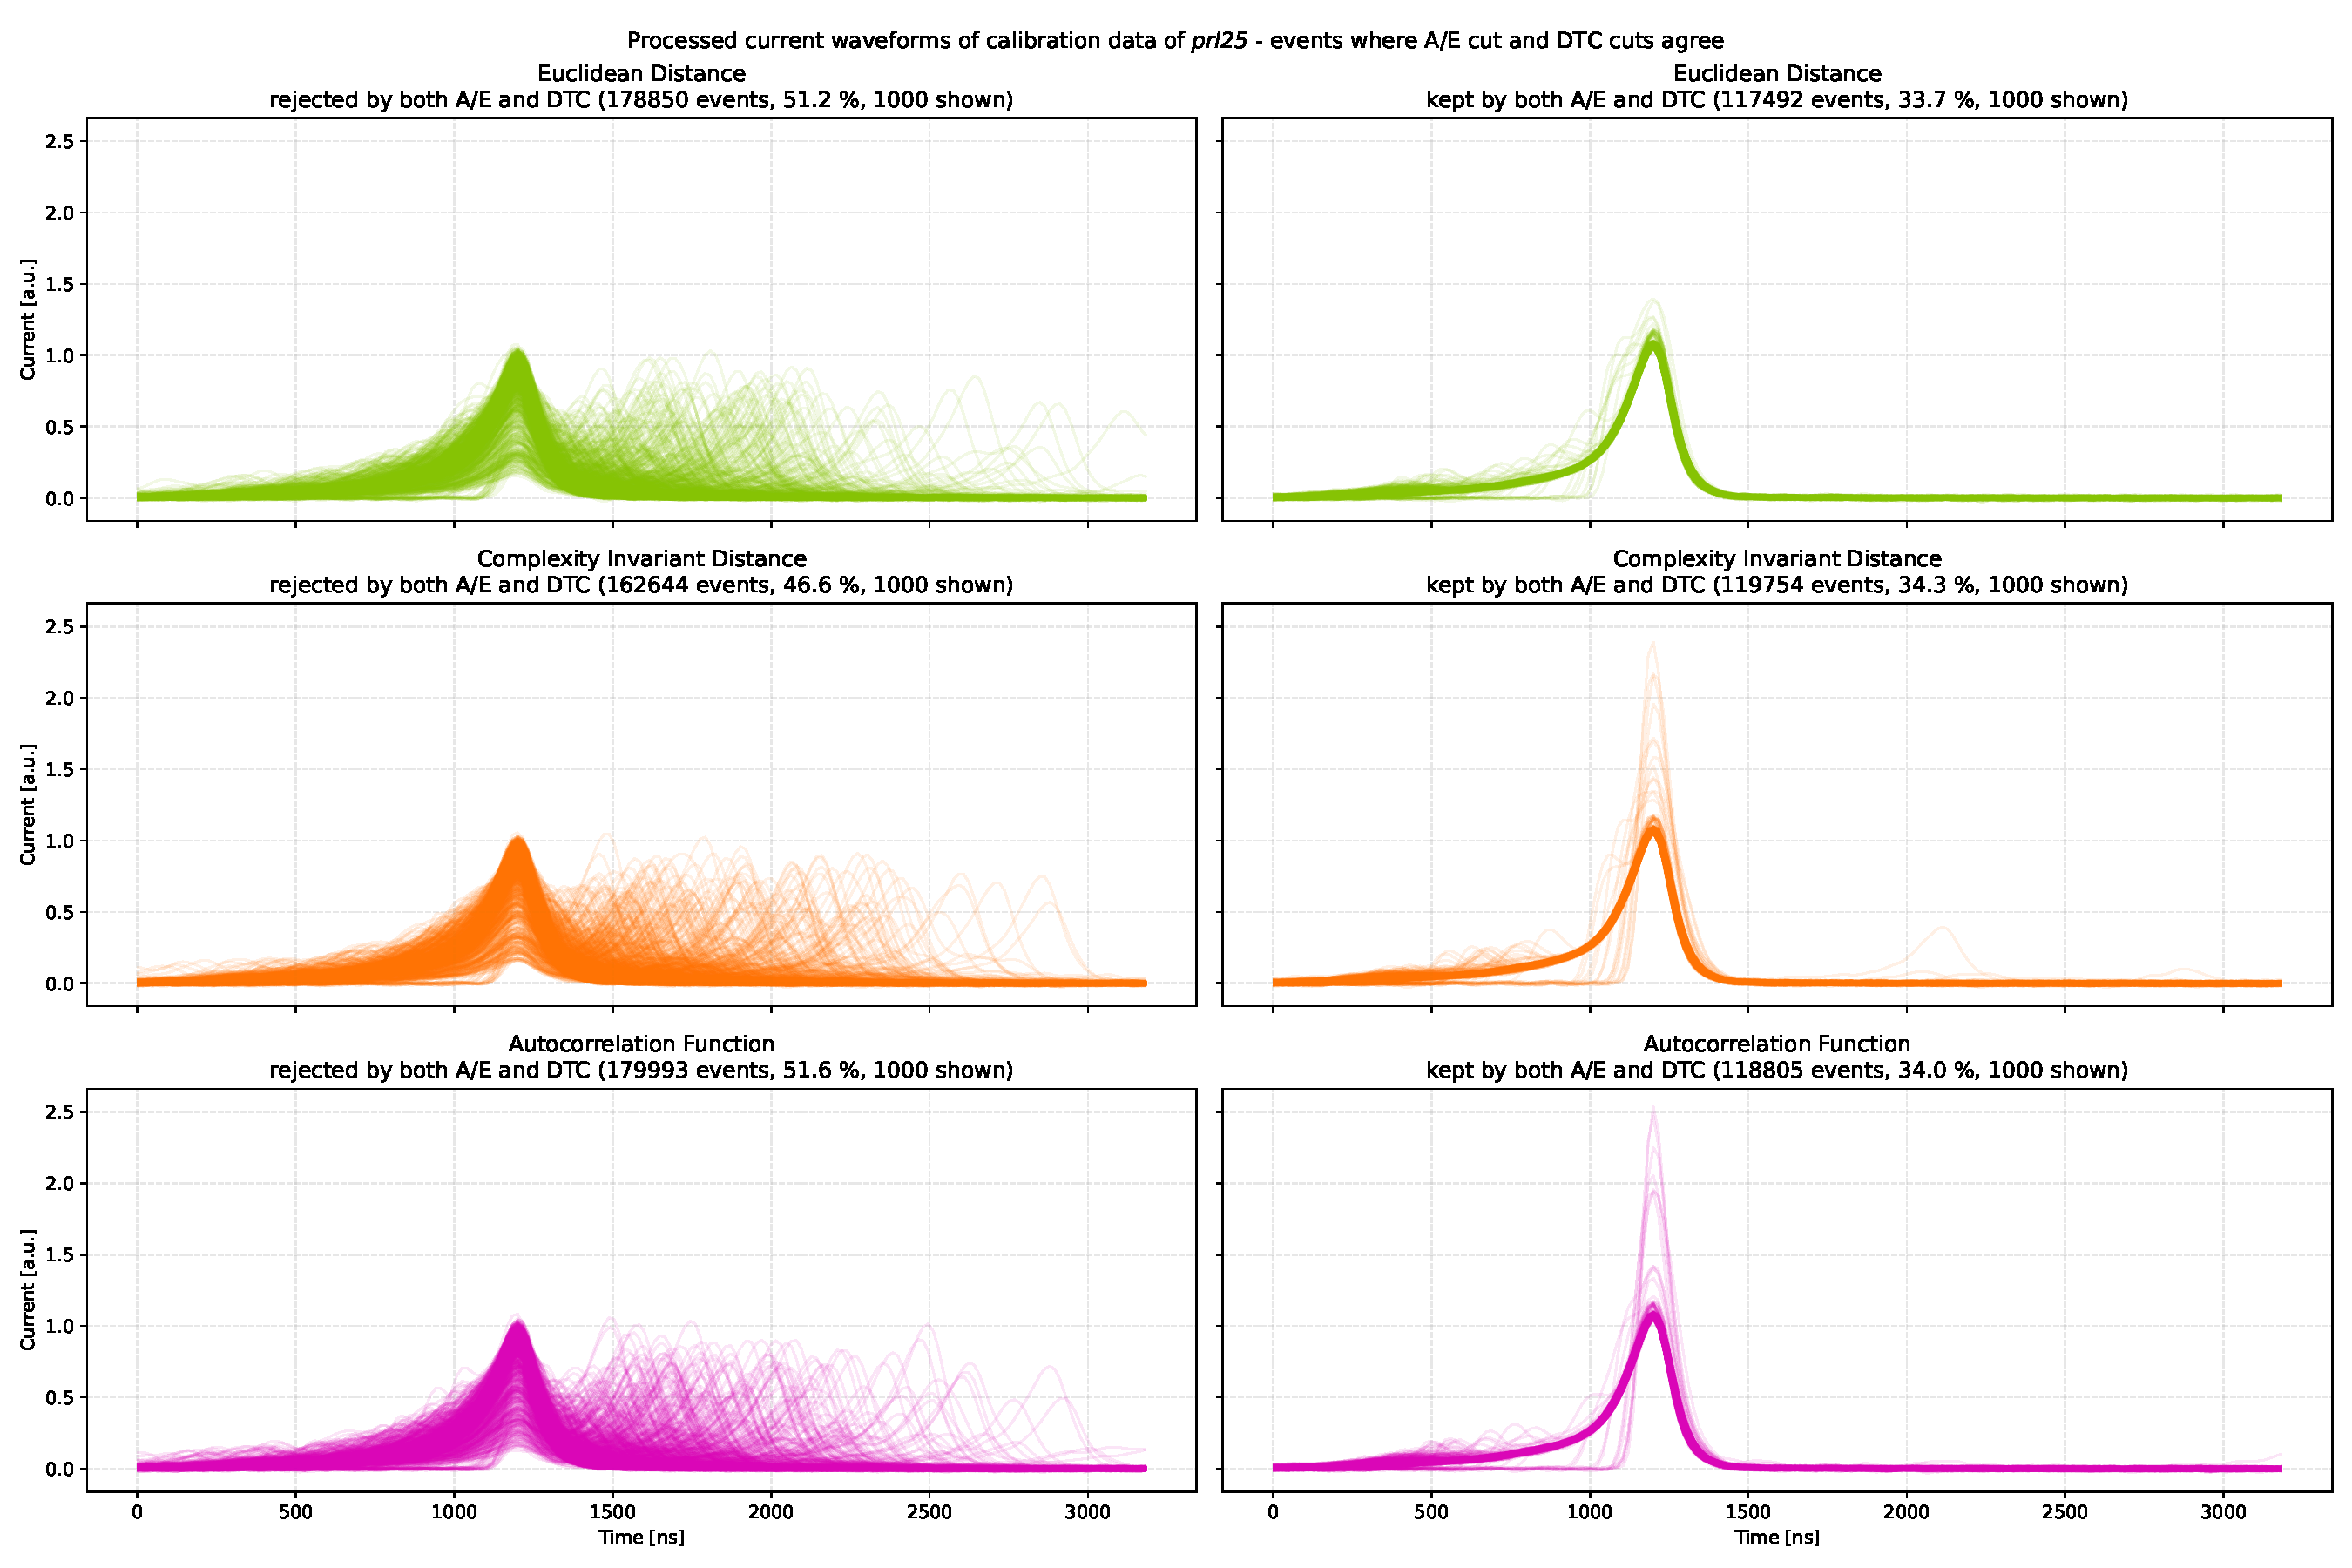
\includegraphics[width=\textwidth]{plots/DTC/all_metrics_calibration_data_agree.pdf}
%     \caption{Waveforms from the \textit{prl25} calibration dataset for which the \ac{AE} and the \ac{DTC} agree.}
%     \label{fig:DTC-waveforms-allmetrics-agree}
% \end{figure}

% \begin{figure}[H]
%     \centering
%     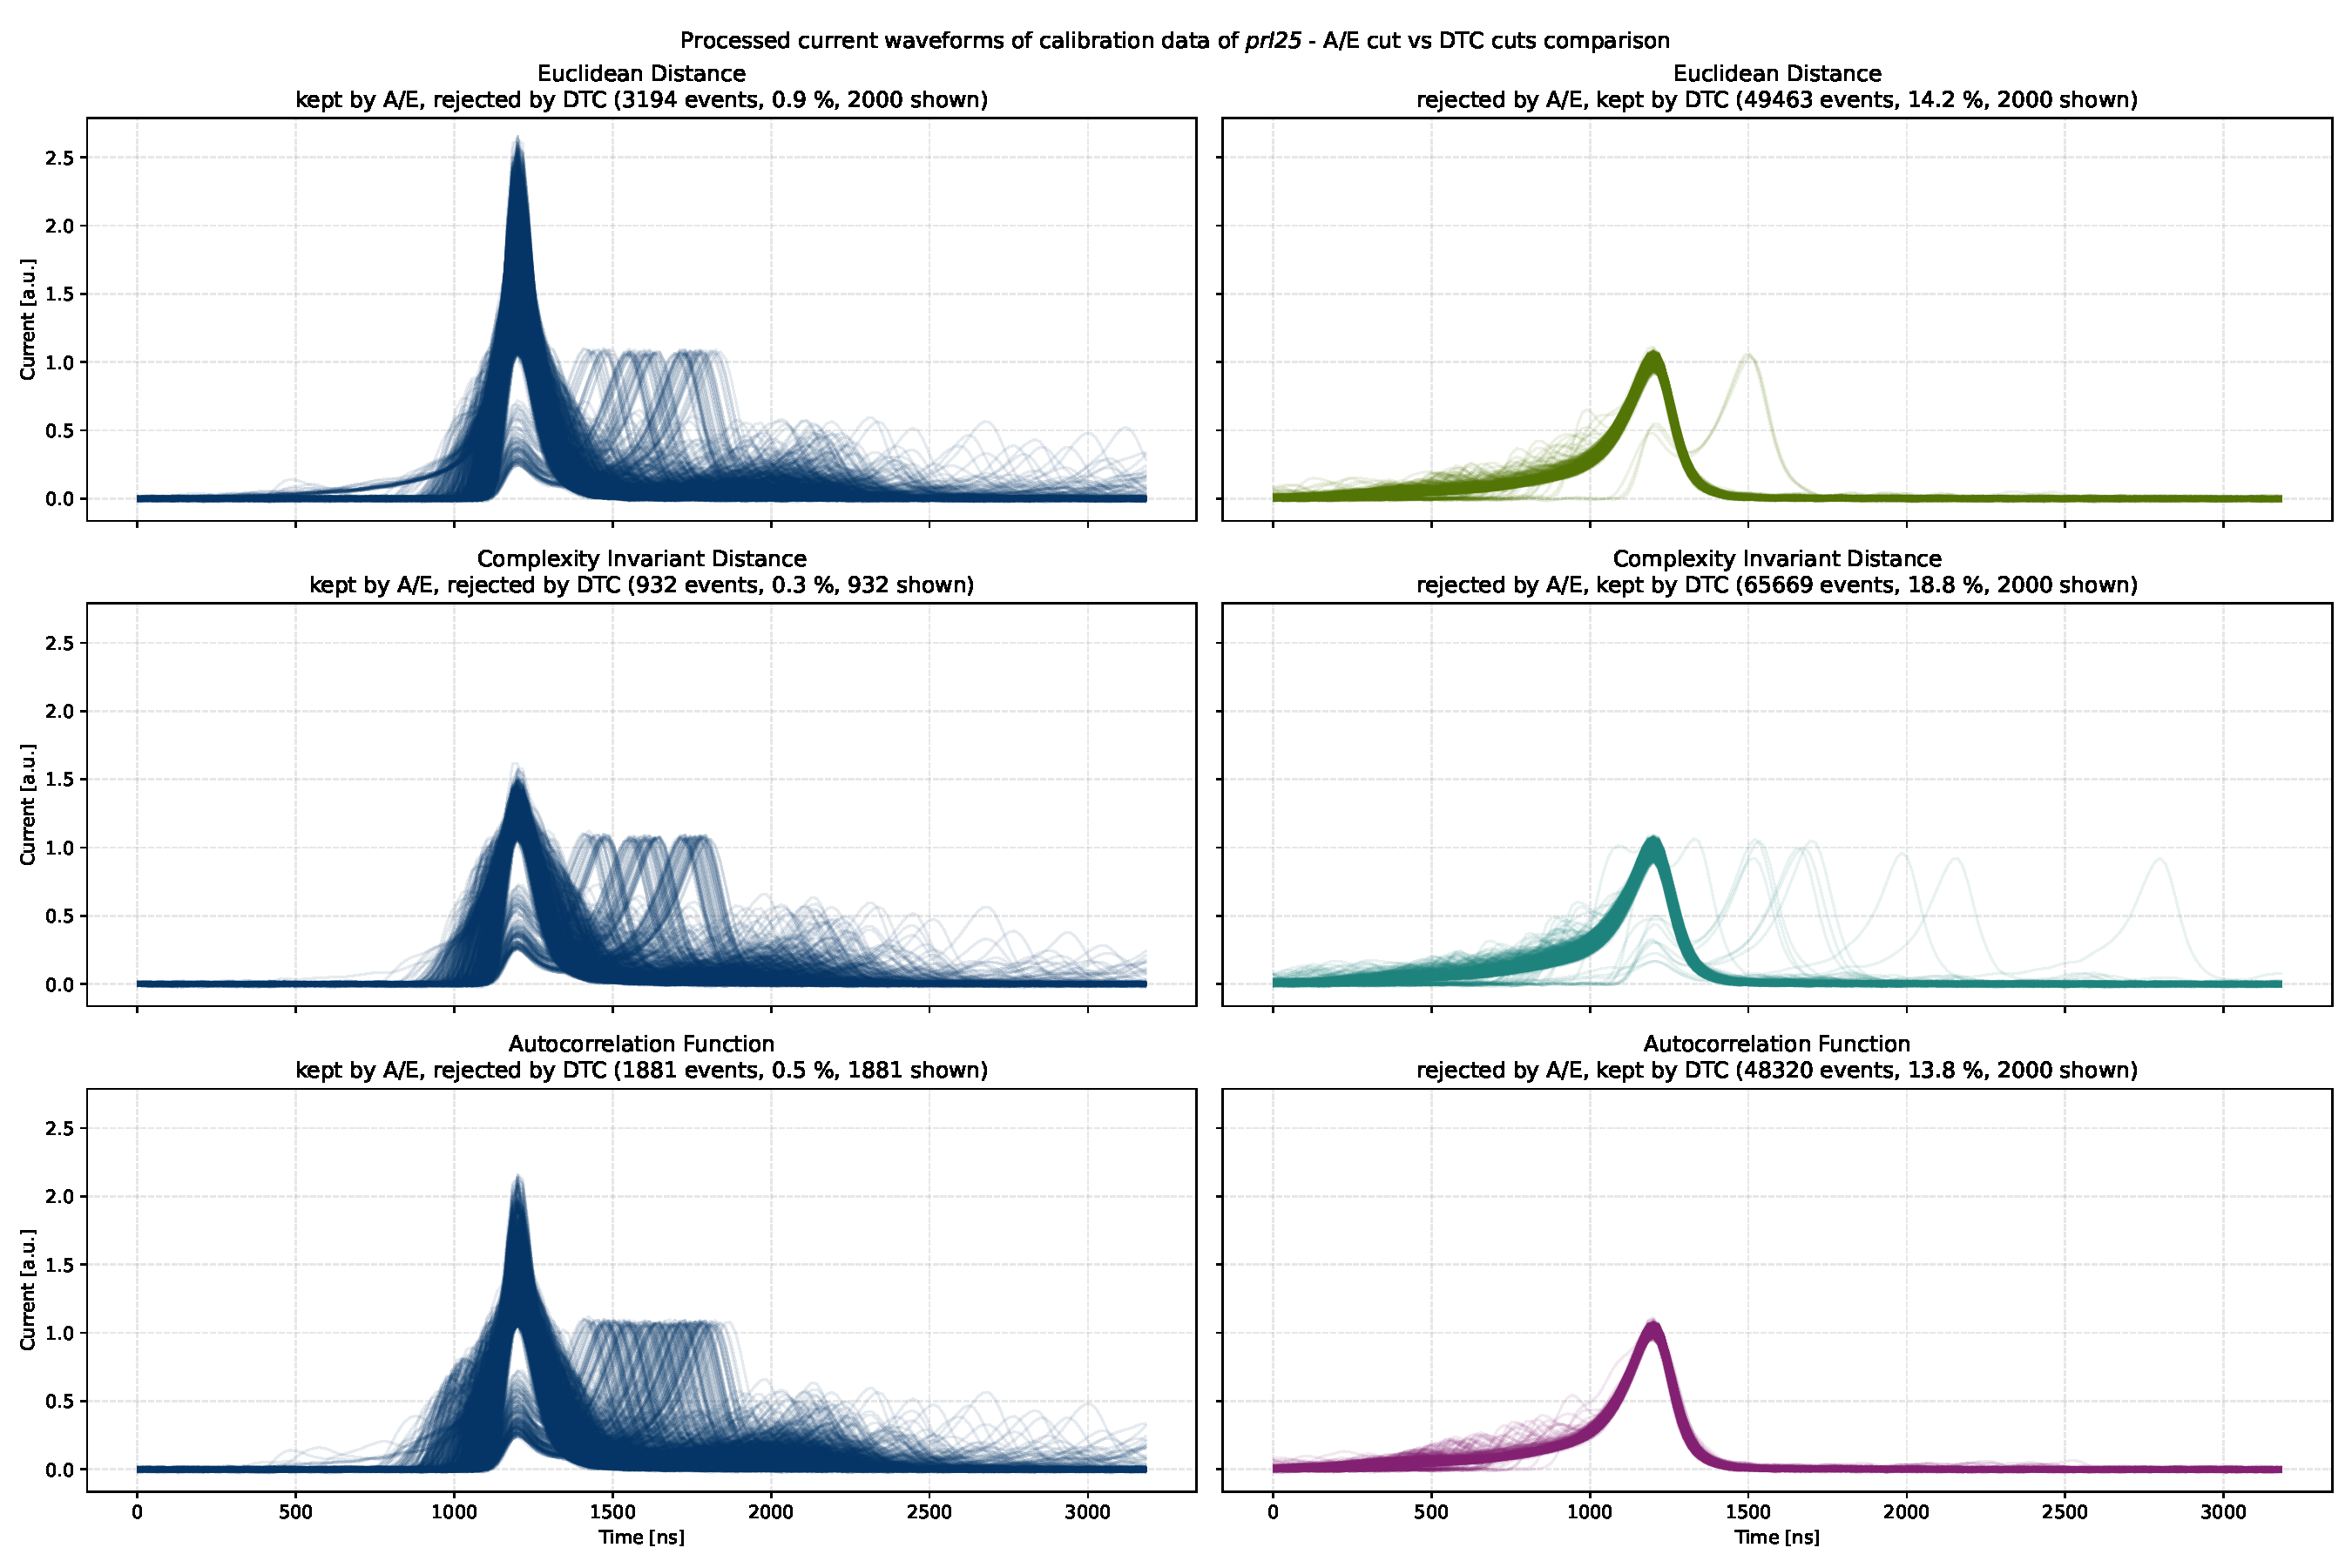
\includegraphics[width=\textwidth]{plots/DTC/all_metrics_calibration_data_disagree.pdf}
%     \caption{Waveforms from the \textit{prl25} calibration dataset for which the \ac{AE} and the \ac{DTC} disagree. }
%     \label{fig:DTC-waveforms-allmetrics-disagree}
% \end{figure}

% \begin{figure}[H]
%     \centering
%     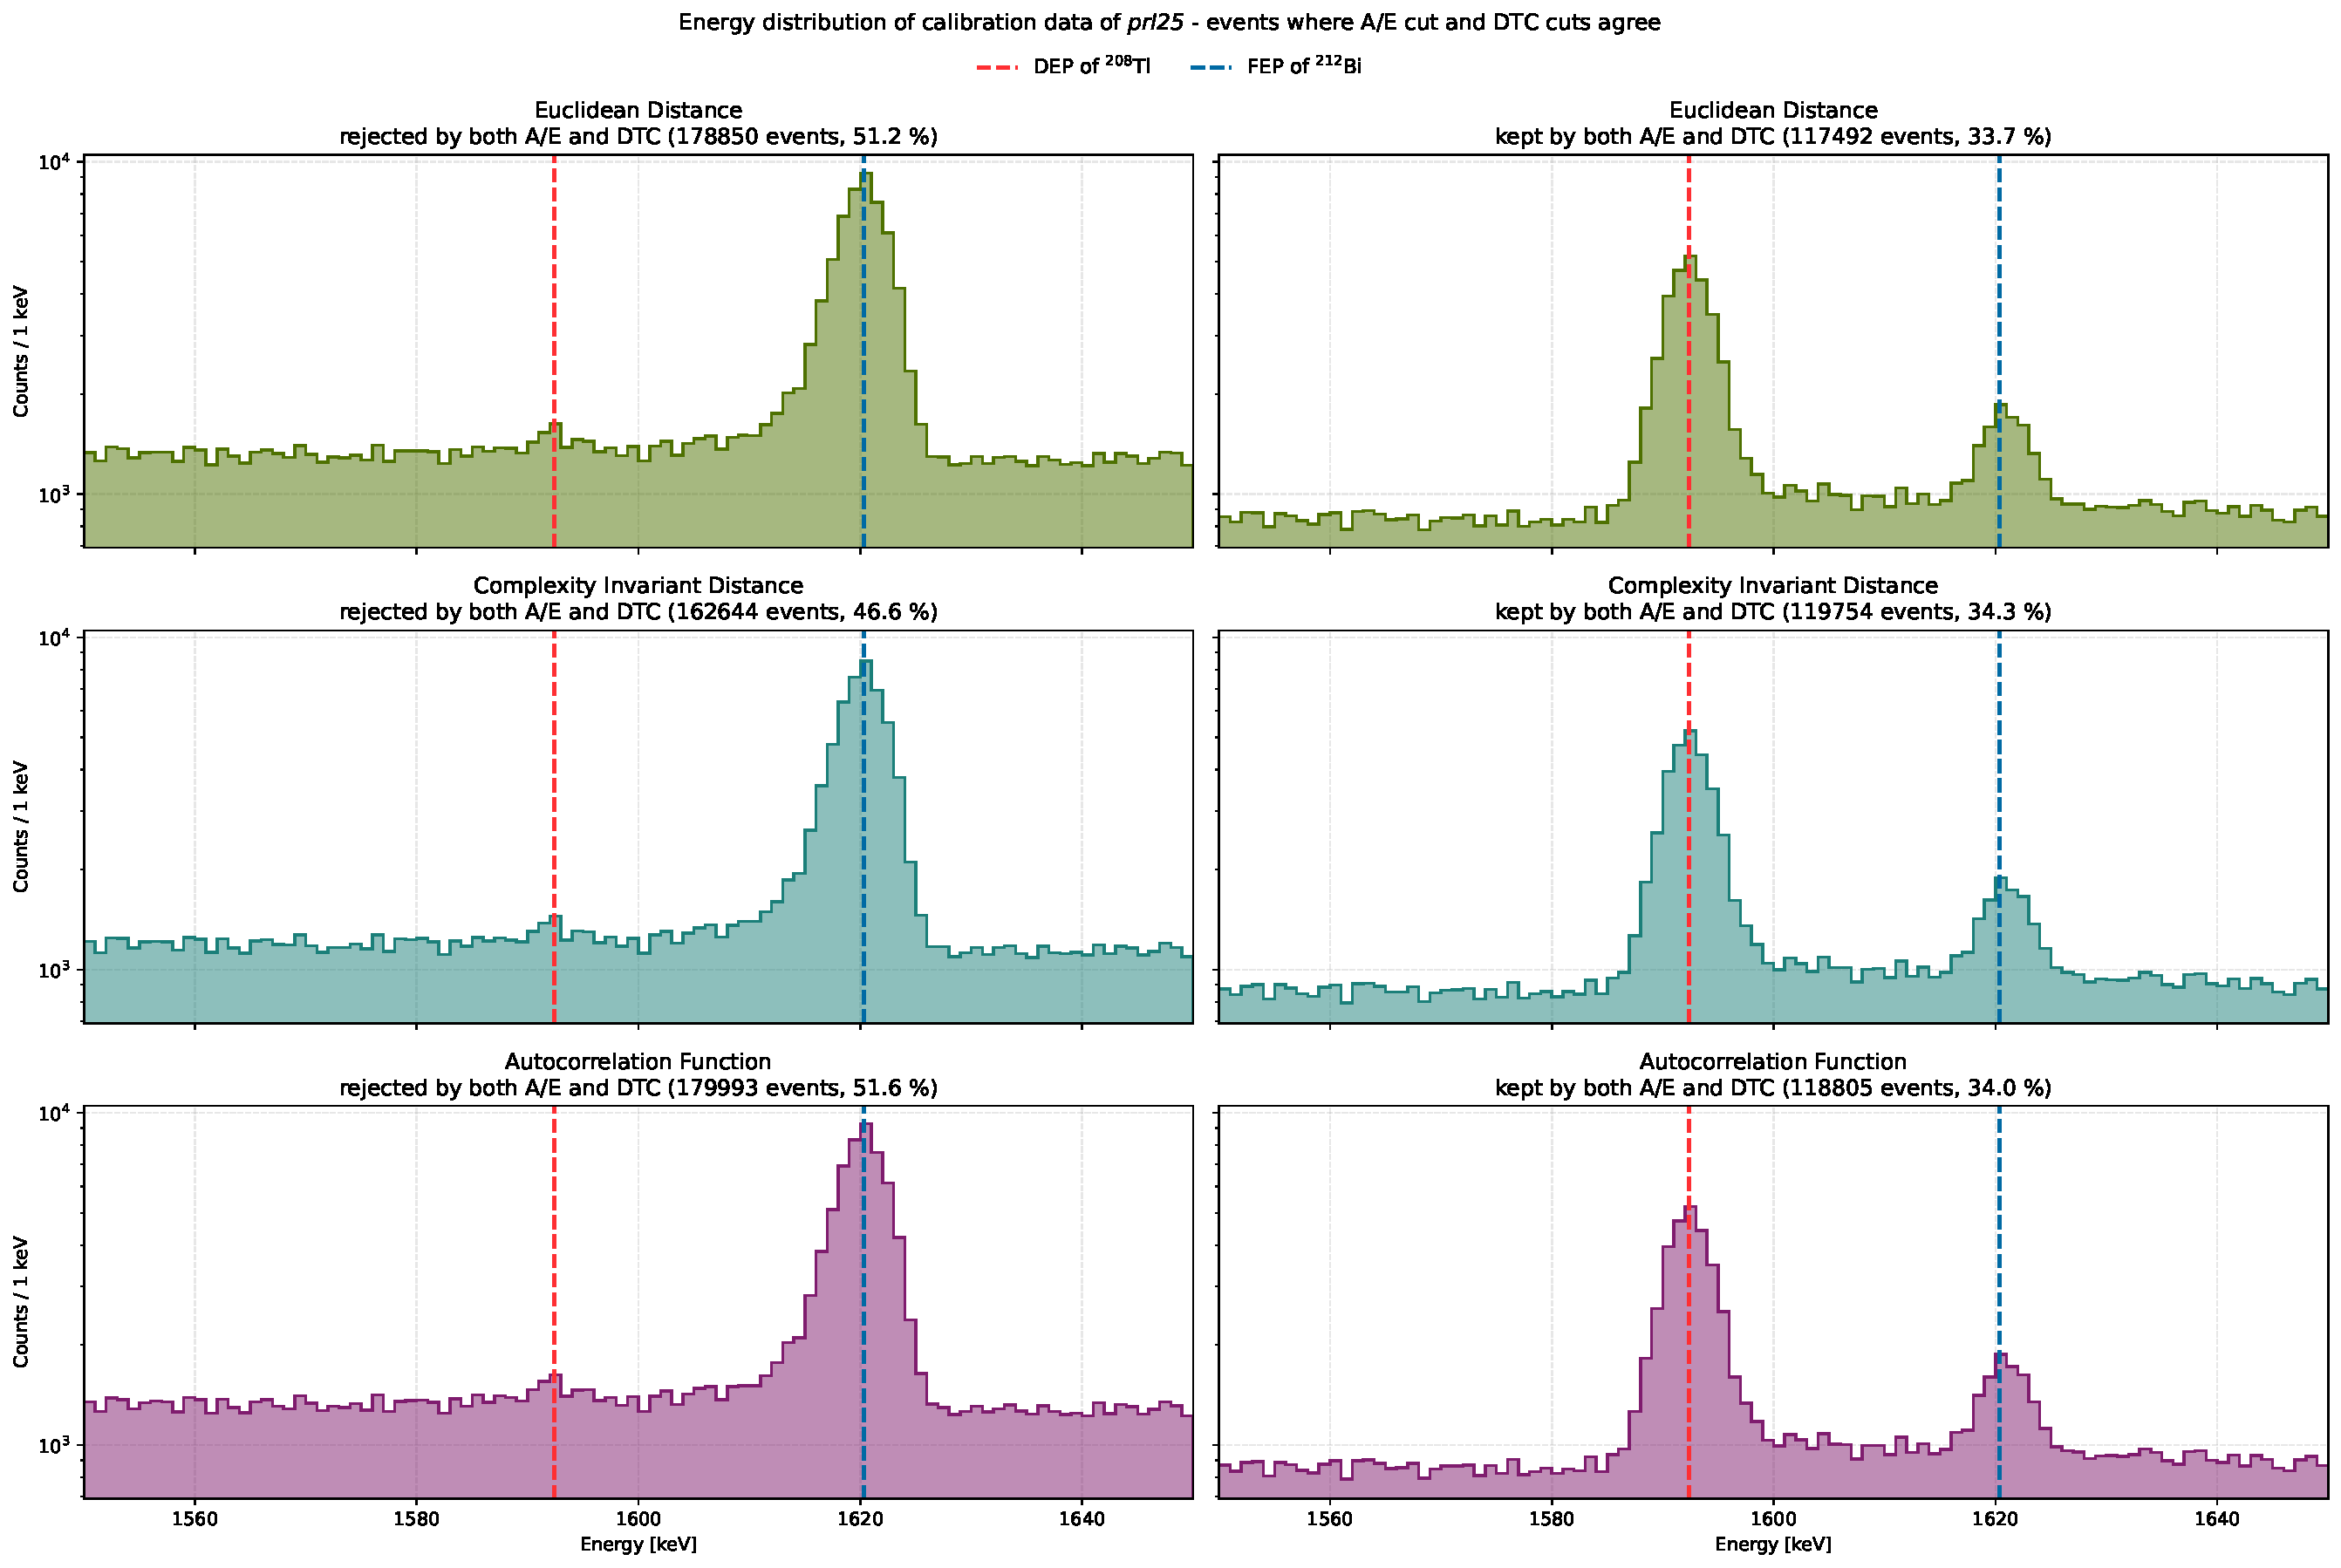
\includegraphics[width=\textwidth]{plots/DTC/all_metrics_calibration_data_agree_energy.pdf}
%     \caption{Energy spectra of waveforms from the \textit{prl25} calibration dataset for which the \ac{AE} and the \ac{DTC} agree.}
%     \label{fig:DTC-waveforms-allmetrics-agree-energy}
% \end{figure}

% \begin{figure}[H]
%     \centering
%     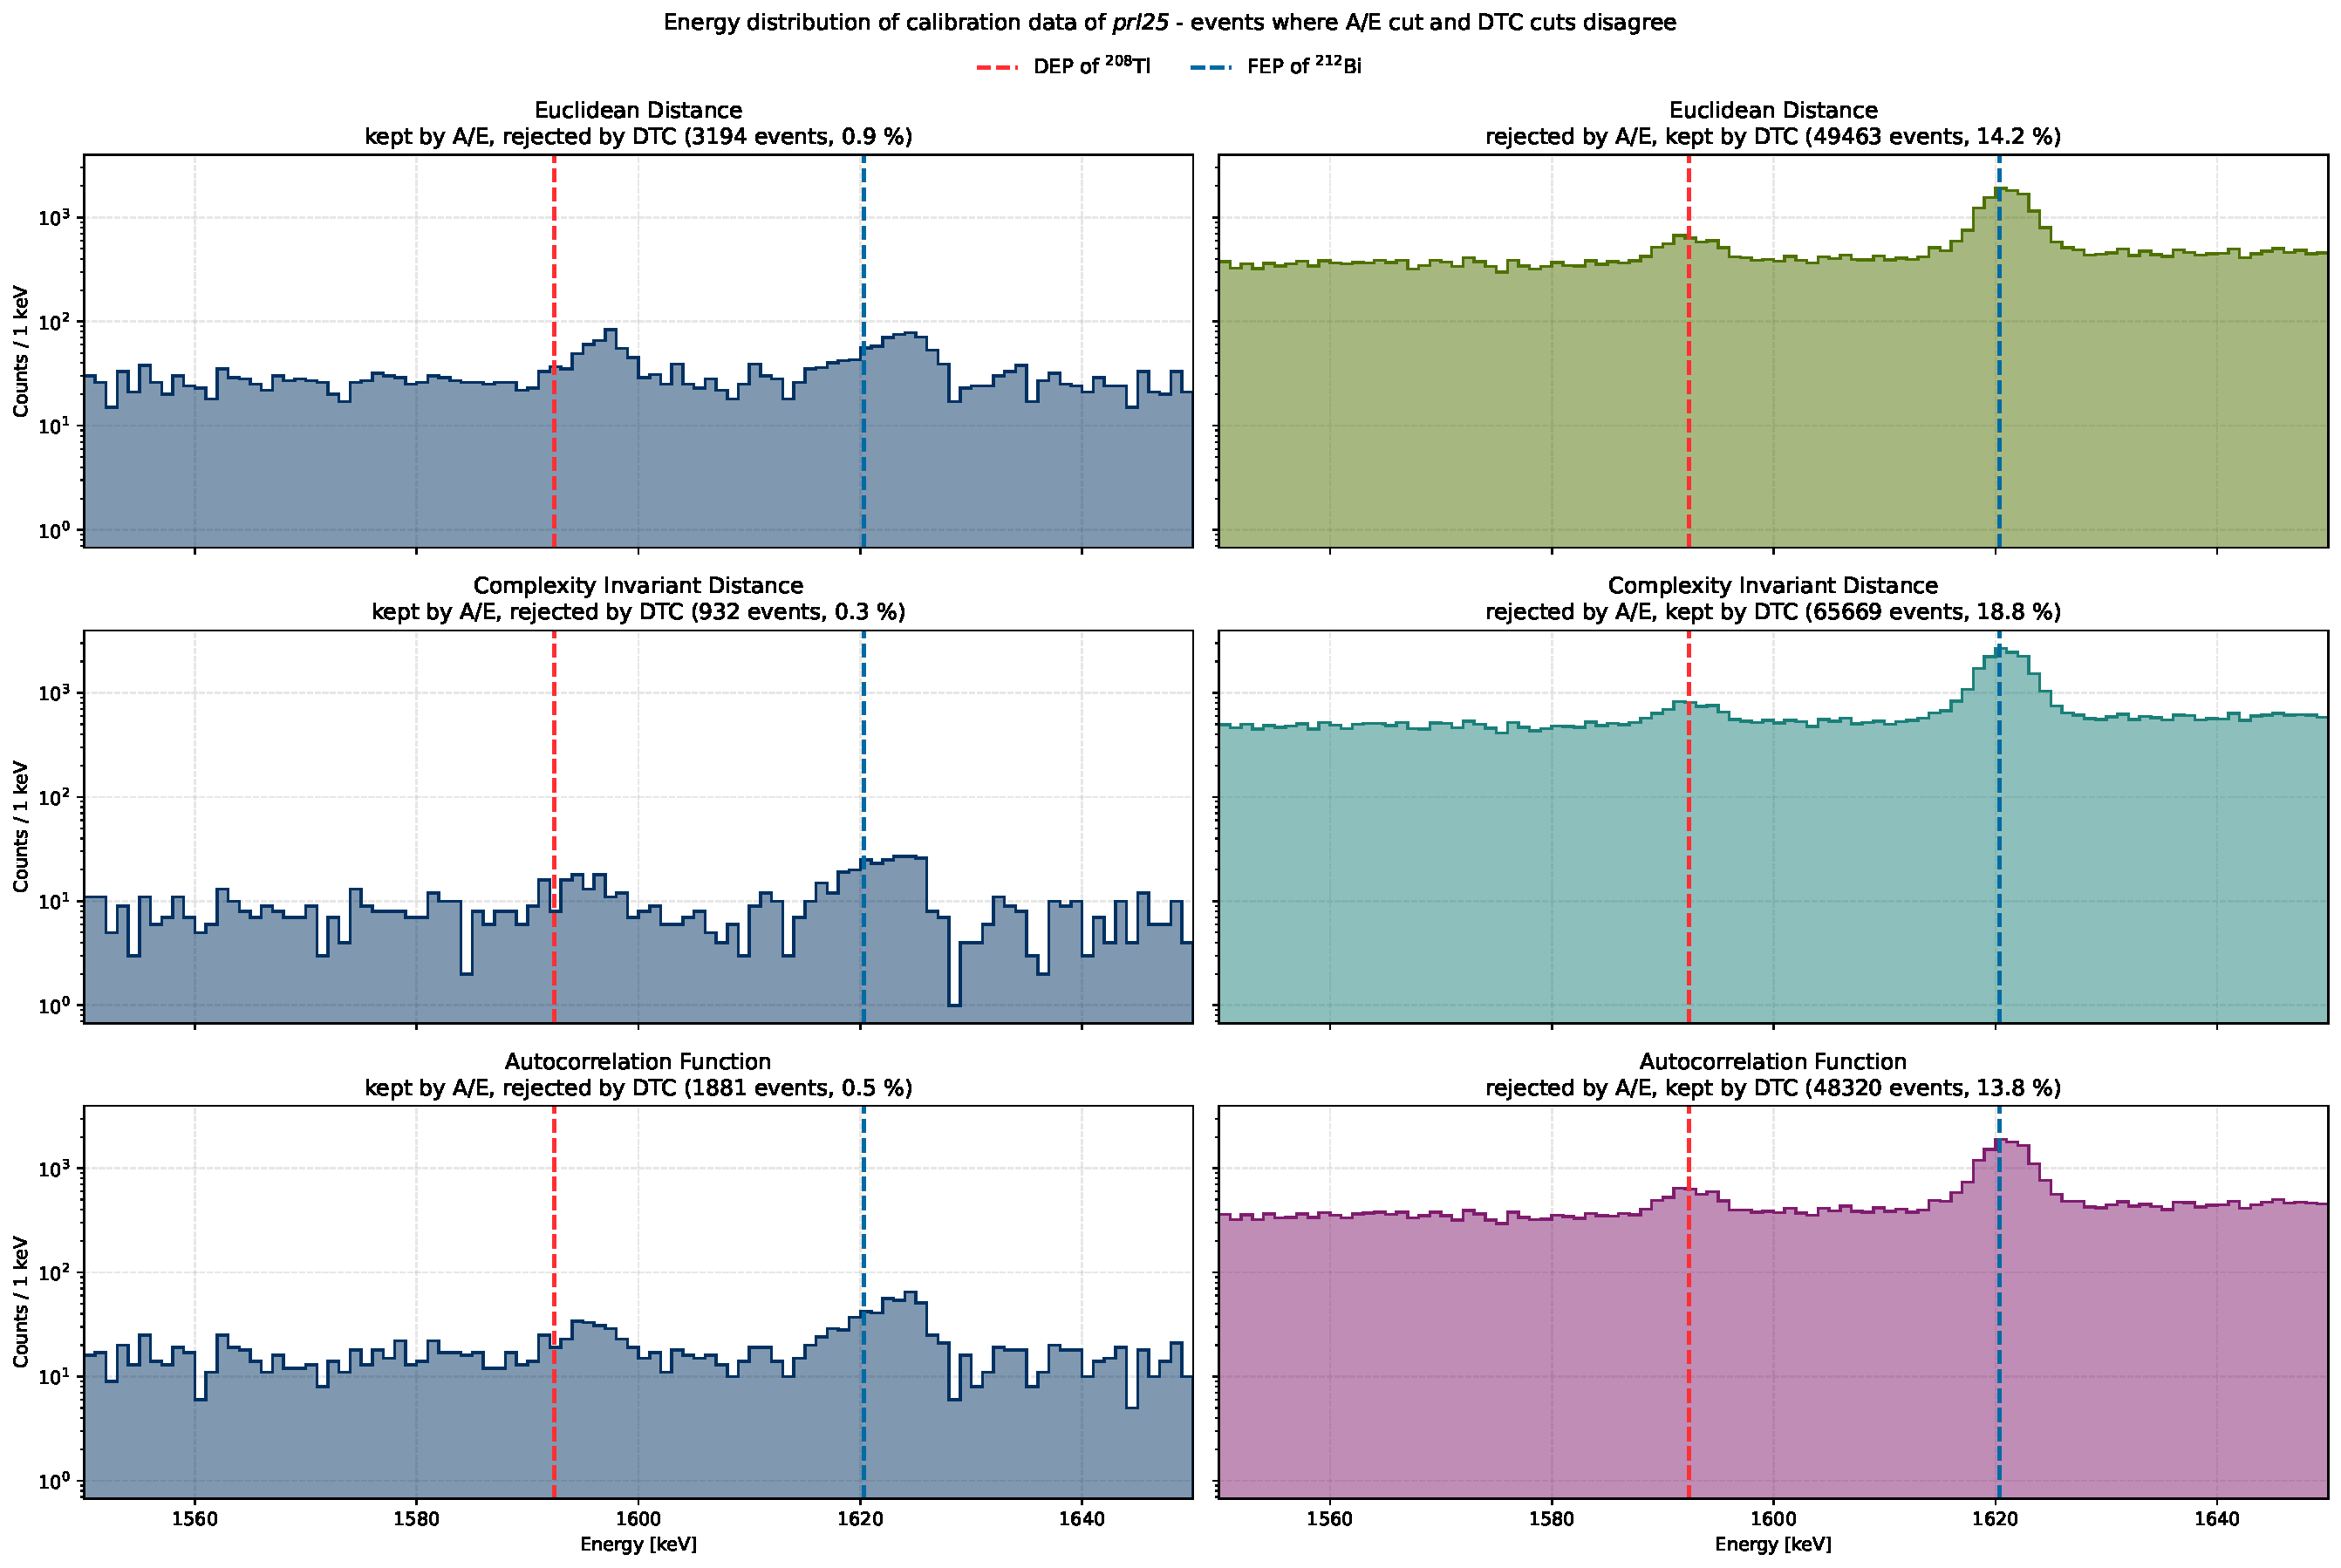
\includegraphics[width=\textwidth]{plots/DTC/all_metrics_calibration_data_disagree_energy.pdf}
%     \caption{Energy spectra of waveforms of the \textit{prl25} calibration dataset for which the \ac{AE} and the \ac{DTC} disagree.}
%     \label{fig:DTC-waveforms-allmetrics-disagree-energy}
% \end{figure}





% ----------------------------------------------------------------------------------
% --------------------------------- 2 NU BETA BETA ---------------------------------
% ----------------------------------------------------------------------------------
% \newpage
% \section{Analysis of~\texorpdfstring{$2\nu\boldsymbol{\beta}\boldsymbol{\beta}$}{2nu beta beta} data}
% \label{sec:2nubb-data}

% The latest step of this analysis involves testing all the deep learning models discussed so far with data that are well-known \ac{SSE}-like events. In particular, physics data from period \textit{p03} to period \textit{p09} of \textit{prl25} have been selected for the V08682A detector. Data are categorized by the \texttt{pygama} pipeline according to whether they qualify as $2\nu\beta\beta$ candidates or not in the range between $560$~keV and $2039$~keV\footnote{Below 556 keV, the spectrum is dominated by~${}^{39}$Ar events.}. On top of that, quality cuts listed in Tab.~\ref{tab:quality-cuts-2nu} have been applied.

% \begin{table}[H]
%     \centering
%     \begin{tabular}{ll}
%         \toprule
%         \textbf{Cut} & \textbf{Filtered events} \\
%         \midrule
%         detector usability      & events recorded while the detector is not flagged as usable (\texttt{usability} $\neq$ \texttt{on}) \\
%         $\beta\beta$-like       & events not flagged as $\beta\beta$-like by the event-level quality selection \\
%         good channel            & hits from channels not flagged as good \\
%         muon veto               & events in coincidence with a muon \\
%         pulser / forced trigger & pulser events and forced-trigger events \\
%         \bottomrule
%     \end{tabular}
%     \caption{Summary of the quality cuts applied to the physics data in the selection of $2\nu\beta\beta$ events.}
%     \label{tab:quality-cuts-2nu}
% \end{table}

% Moreover, data have been cut on the basis of the \ac{lar} veto, as shown in Fig.~\ref{fig:2nu-beforeafterLAR}. In principle, the resulting spectrum should be made up of pure \ac{SSE}-like events, since all the background contamination producing \ac{MSE} signals are removed by the \ac{lar} and muon veto. Therefore, all of the models discussed in Chapter~\ref{chapter:ML-PSD} and trained on calibration data have been all applied to this novel dataset, without any further training, to test wheter they recognised as signal-like events or not.
% \begin{figure}[H]
%     \centering
%     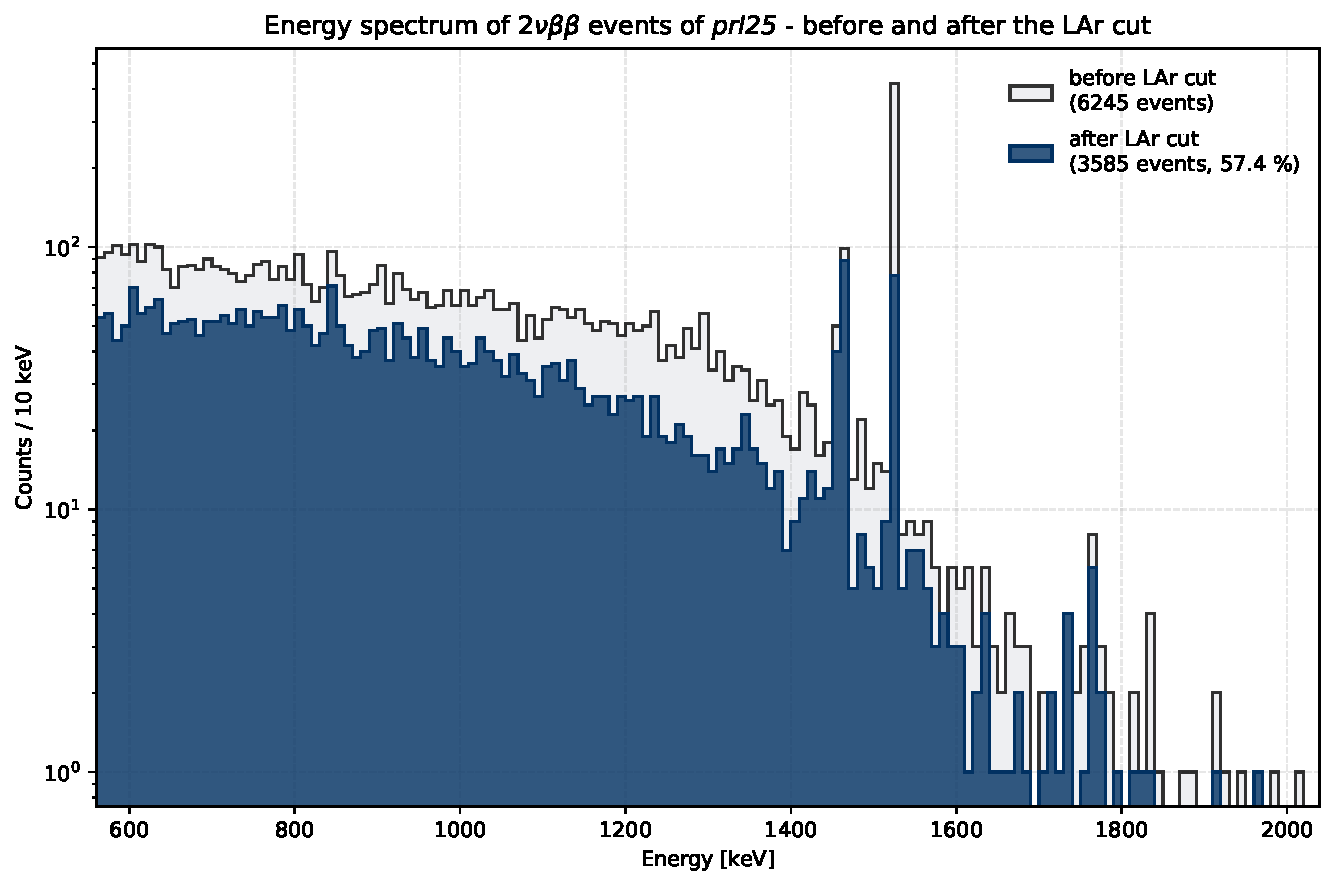
\includegraphics[width=0.8\textwidth]{plots/2nubb/energy_spectrum_before_after_LAr.pdf}
%     \caption{Energy spectrum of the $2\nu\beta\beta$ data before (light grey) and after (dark grey) the \ac{lar} cut.}
%     \label{fig:2nu-beforeafterLAR}
% \end{figure}

% \subsection{\texorpdfstring{\acs{VAE}}{VAE}-based classifier}

% \subsection{\texorpdfstring{\acs{DTC}}{DTC}}




% \begin{figure}[H]
%     \centering
%     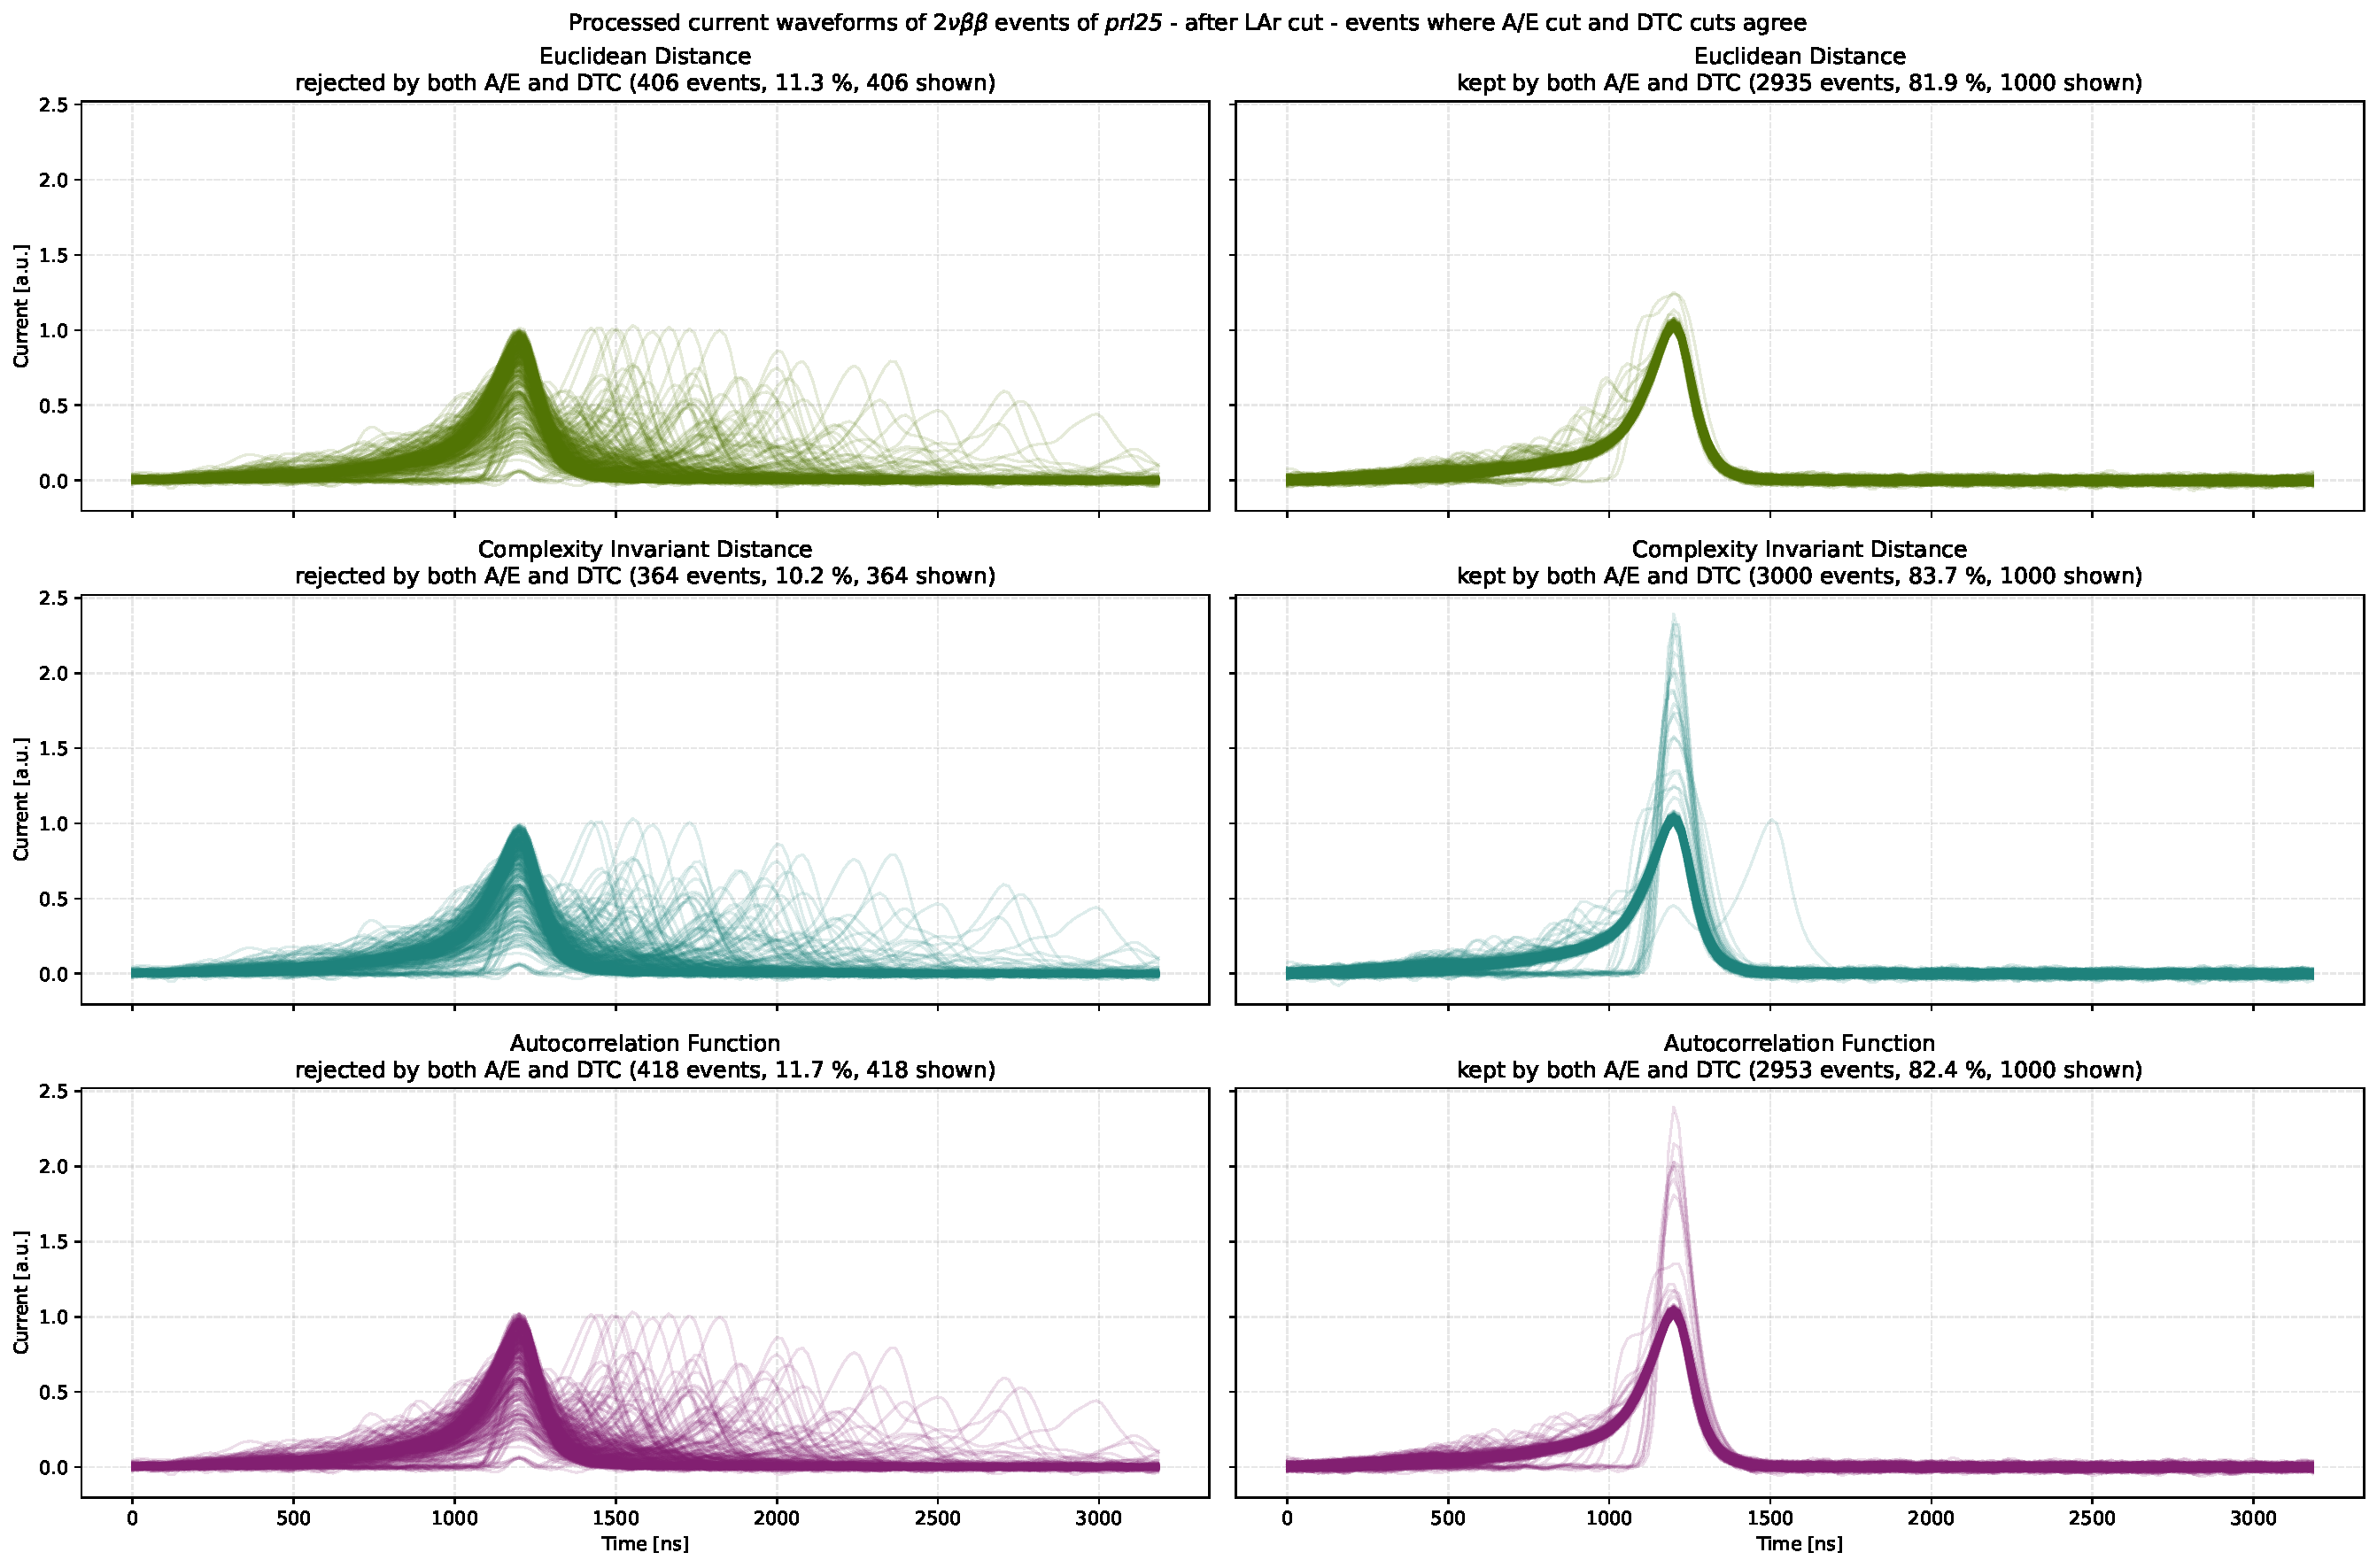
\includegraphics[width=\textwidth]{plots/2nubb/waveforms_AoE_DTC_agree_afterLAr.pdf}
%     \caption{Current waveforms kept (right) and rejected (left) by both the \ac{AE} cut and the \ac{DTC} algorithm. From the top to the bottom Euclidean Distance, Complexity Invariant Distance and Autocorrelation Function.}
%     \label{fig:2nu-kept_rejected_AE_DTC_agree}
% \end{figure}

% \begin{figure}[H]
%     \centering
%     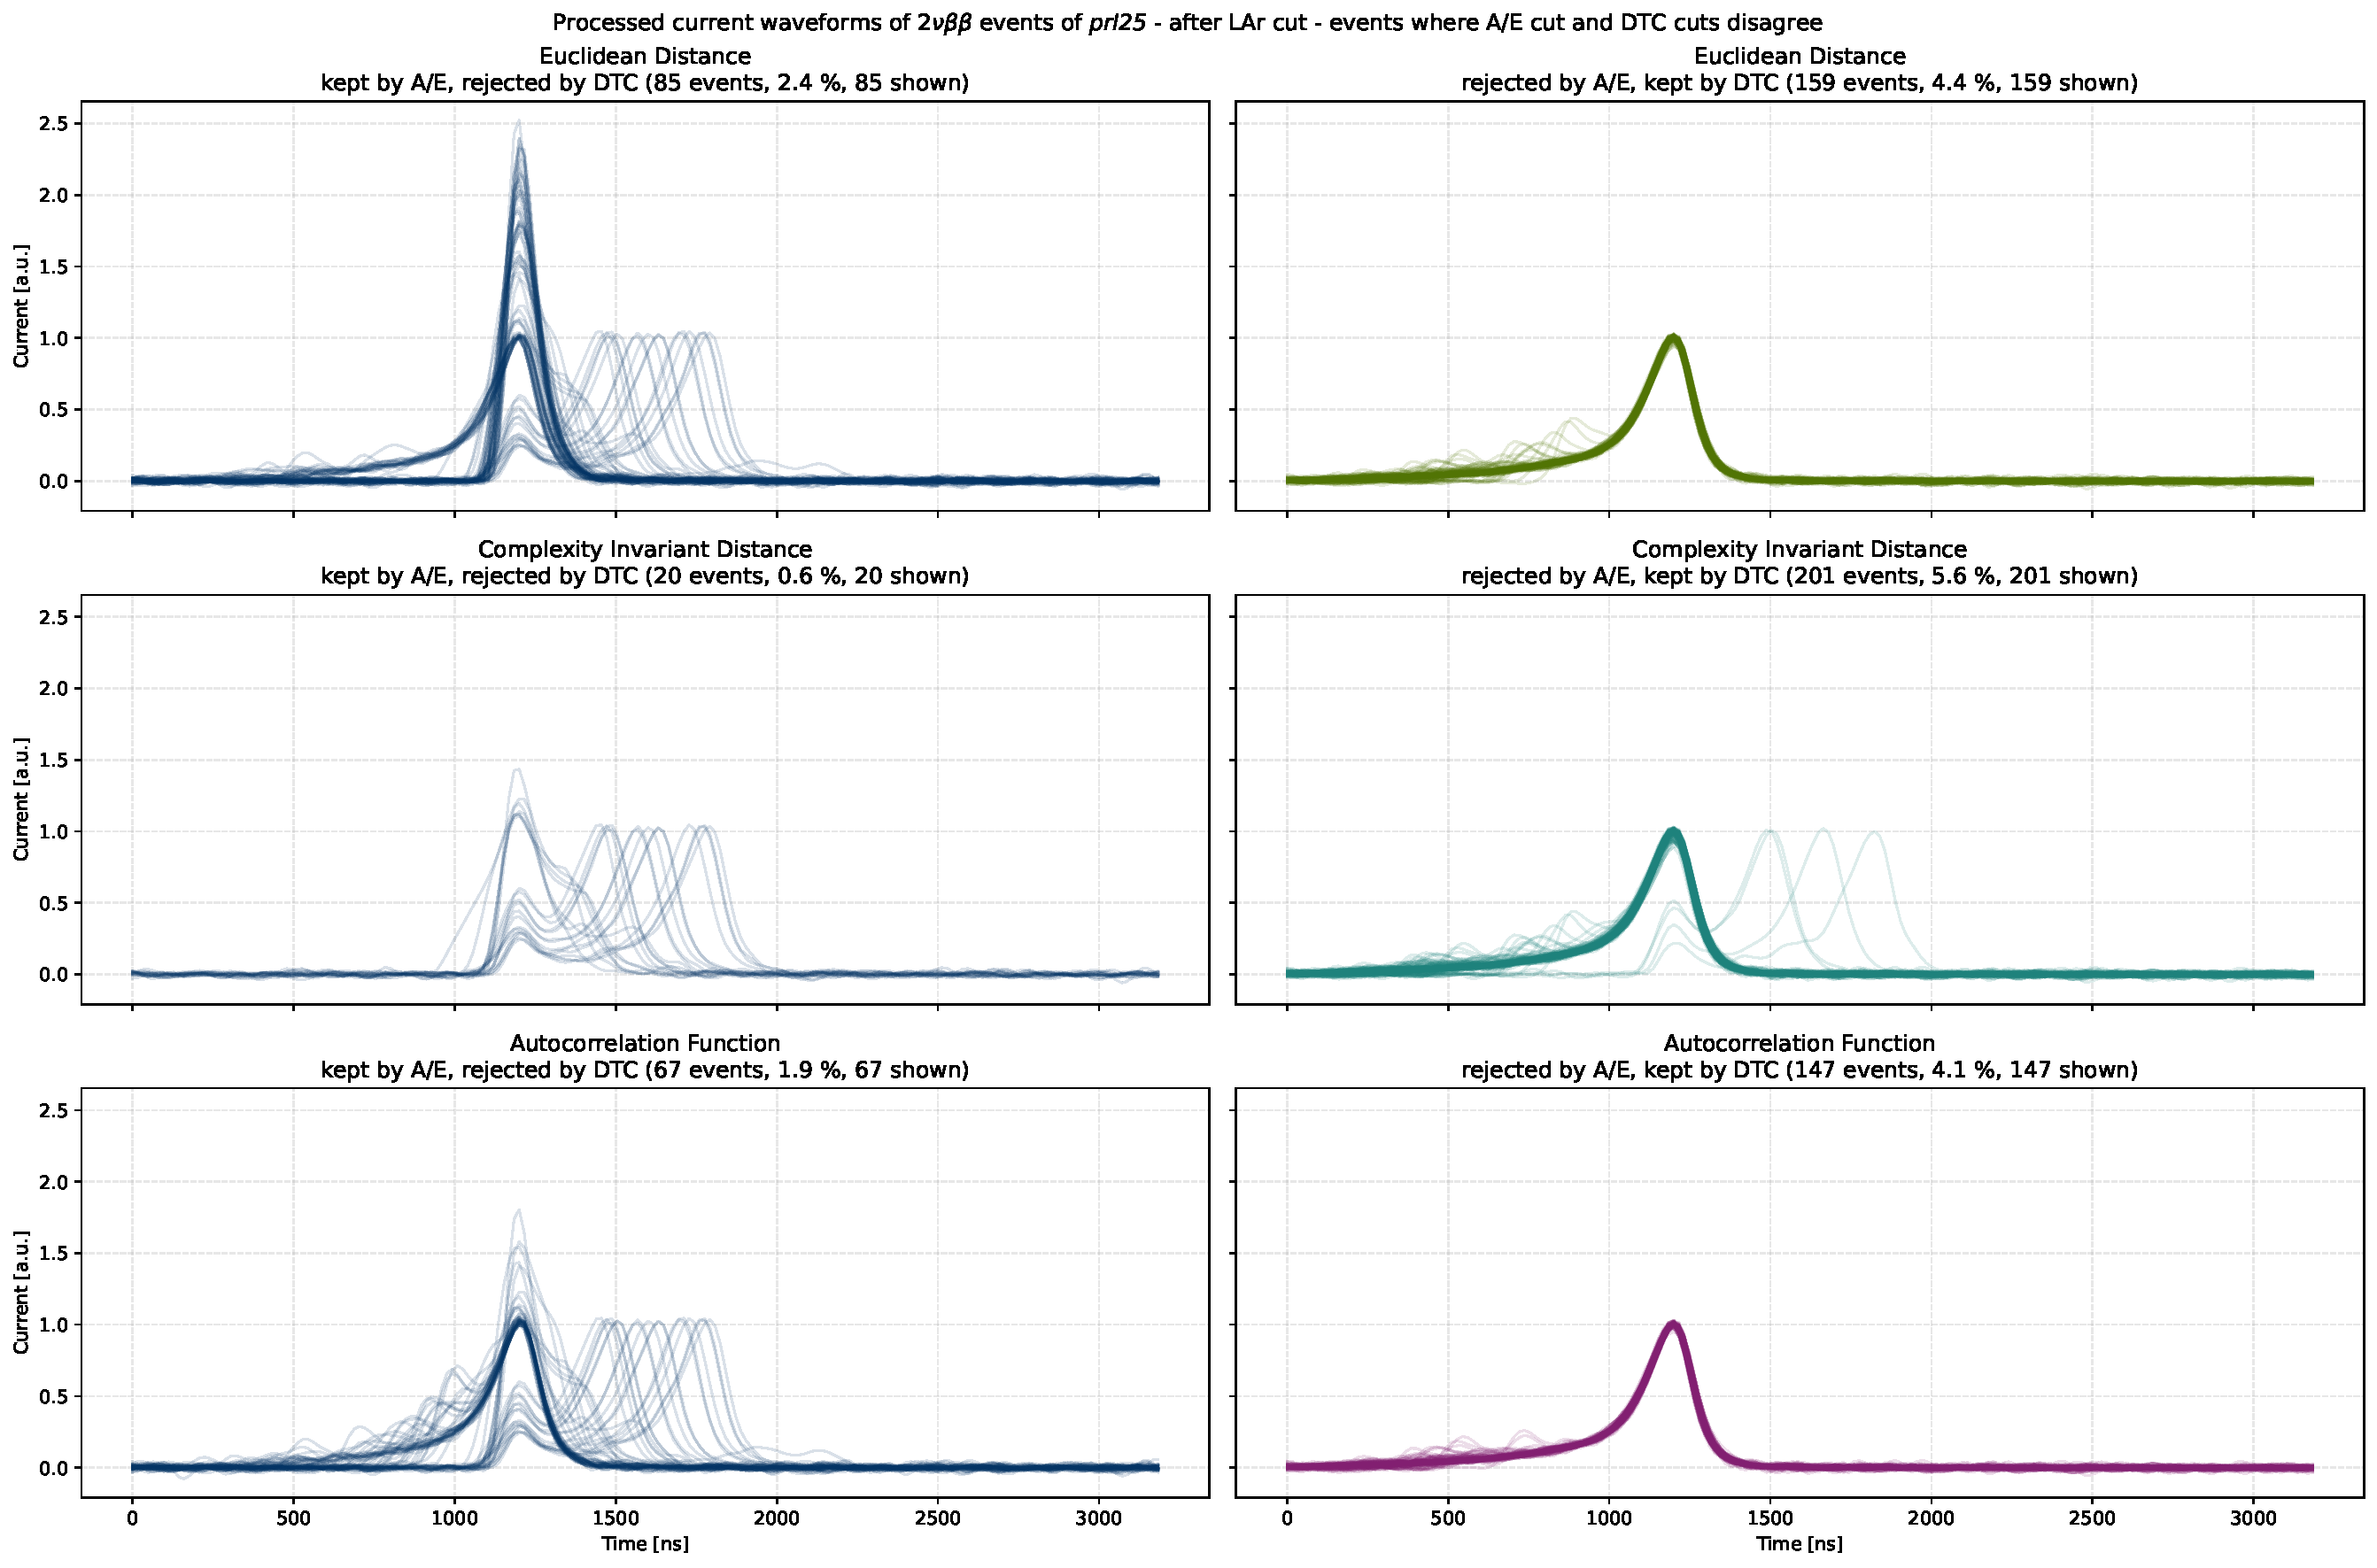
\includegraphics[width=\textwidth]{plots/2nubb/waveforms_AoE_DTC_disagree_afterLAr.pdf}
%     \caption{Comparison between current waveforms kept and rejectd by different cuts: On th eleft waveforms kept by the \ac{AE} cut but rejected by a specific \ac{DTC} metric cut, viceversa on the right events rejected by the \ac{DTC} metric but kept by \ac{AE} are shown. From the top to the bottom Euclidean Distance, Complexity Invariant Distance and Autocorrelation Function.}
%     \label{fig:2nu-kept_rejected_AE_DTC_disagree}
% \end{figure}